% To compile this document, just run pdflatex first-known-goat-grazing-problem.tex.
% If you're using TeXShop, typeset it using the LaTeX command.
% Don't run bibtex on the document. You'll get errors as there are no references.
\documentclass{article}

\usepackage{amsmath}					% For the aligned environment
\usepackage{csquotes}					% For the displayquote environment
\usepackage{graphicx}					% For \includegraphics
\usepackage[margin=1in]{geometry}
\usepackage{titling}						% For \predate, \postdate, \preauthor and \postauthor

% The following two packages are for \url and for breaking long URLs at hyphens.
% If you don't want to break long URLs but want them formatted, use just hyperref.
% If you only want to break long URLs but don't want to format them, use just xurl.
\usepackage{xurl}
\usepackage{hyperref}

\usepackage{xstring}
\let\oldtexttt\texttt
\renewcommand{\texttt}[1]{\oldtexttt{\StrSubstitute[0]{#1}{-}{\allowbreak-\allowbreak}}}
	% Source: https://tex.stackexchange.com/questions/299/how-to-get-long-texttt-sections-to-break
	% 	Archived at: https://archive.ph/iKOZE

\newcommand{\texttttilde}{\raisebox{0.5ex}{\oldtexttt{\texttildelow}}}
	% Source: https://tex.stackexchange.com/questions/9363/how-does-one-insert-a-backslash-or-a-tilde-into-latex
	% 	Archived at: https://archive.ph/llem4

\predate{}
\date{}
\postdate{}

\preauthor{}
\postauthor{}

\title{The First Known Goat Grazing Problem}

\begin{document}

\maketitle

I learnt about the first known goat grazing problem from the following article in Quanta Magazine: \url{https://quantamagazine.org/after-centuries-a-seemingly-simple-math-problem-gets-an-exact-solution-20201209/} (archived at: \url{https://archive.ph/lnhUn}). The article states:

\begin{displayquote}
The first problem of this type was published in the 1748 issue of the London-based periodical \textit{The Ladies Diary: Or, The Woman's Almanack} -- a publication that promised to present ``new improvements in arts and sciences, and many diverting particulars.''

The original scenario involves ``a horse tied to feed in a Gentlemen's Park.'' In this case, the horse is tied to the outside of a circular fence. If the length of the rope is the same as the circumference of the fence, what is the maximum area upon which the horse can feed? This version was subsequently classified as an ``exterior problem,'' since it concerned grazing outside, rather than inside, the circle.

An answer appeared in the \textit{Diary}'s 1749 edition. It was furnished by ``Mr. Heath,'' who relied upon ``Trial and a Table of Logarithms,'' among other resources, to reach his conclusion.

Heath's answer -- 76,257.86 square yards for a 160-yard rope -- was an approximation rather than an exact solution. To illustrate the difference, consider the equation $x^2 - 2 = 0$. One could derive an approximate numerical answer, $x = 1.4142$, but that's not as accurate or satisfying as the exact solution, $x = \sqrt{2}$.
\end{displayquote}

In this document, I explain why Mr. Heath might have had to resort to numerical methods to solve this problem.

To be able to compute the maximum area in which the horse can graze, we need to find the equation of the curve traced by the maximum extent of the rope. This curve is shown in the Quanta Magazine article (see the second last image in the article proper). The image from the article that shows the curve can be seen below:

\begin{figure}[h]
% 0.38999176
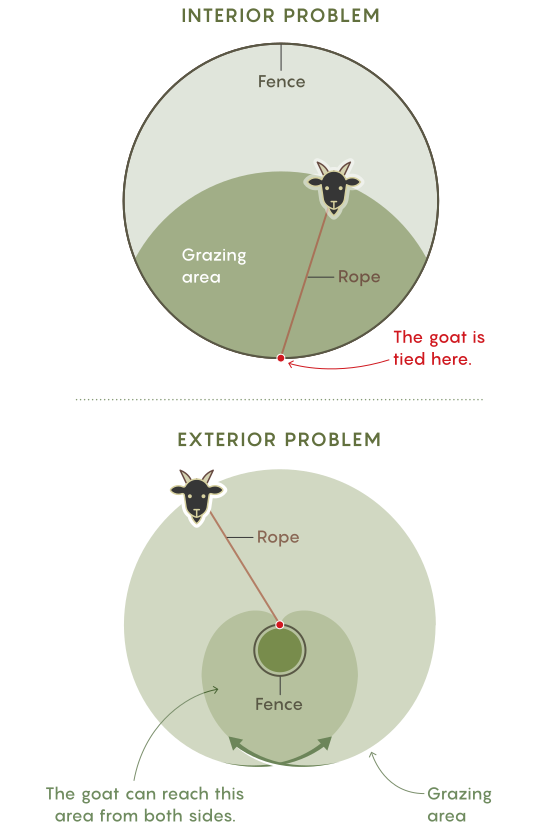
\includegraphics[scale=0.35]{Grazing-goat-figure}
\centering
\end{figure}

The situation we are considering here can be seen in the "Exterior Problem" part of the image. The image in the article is in SVG format. I converted it to PNG using GIMP because the \textbackslash includegraphics\{\} command doesn't work with SVG images.

The following diagram shows the setup we'll be using:

\begin{figure}[h]
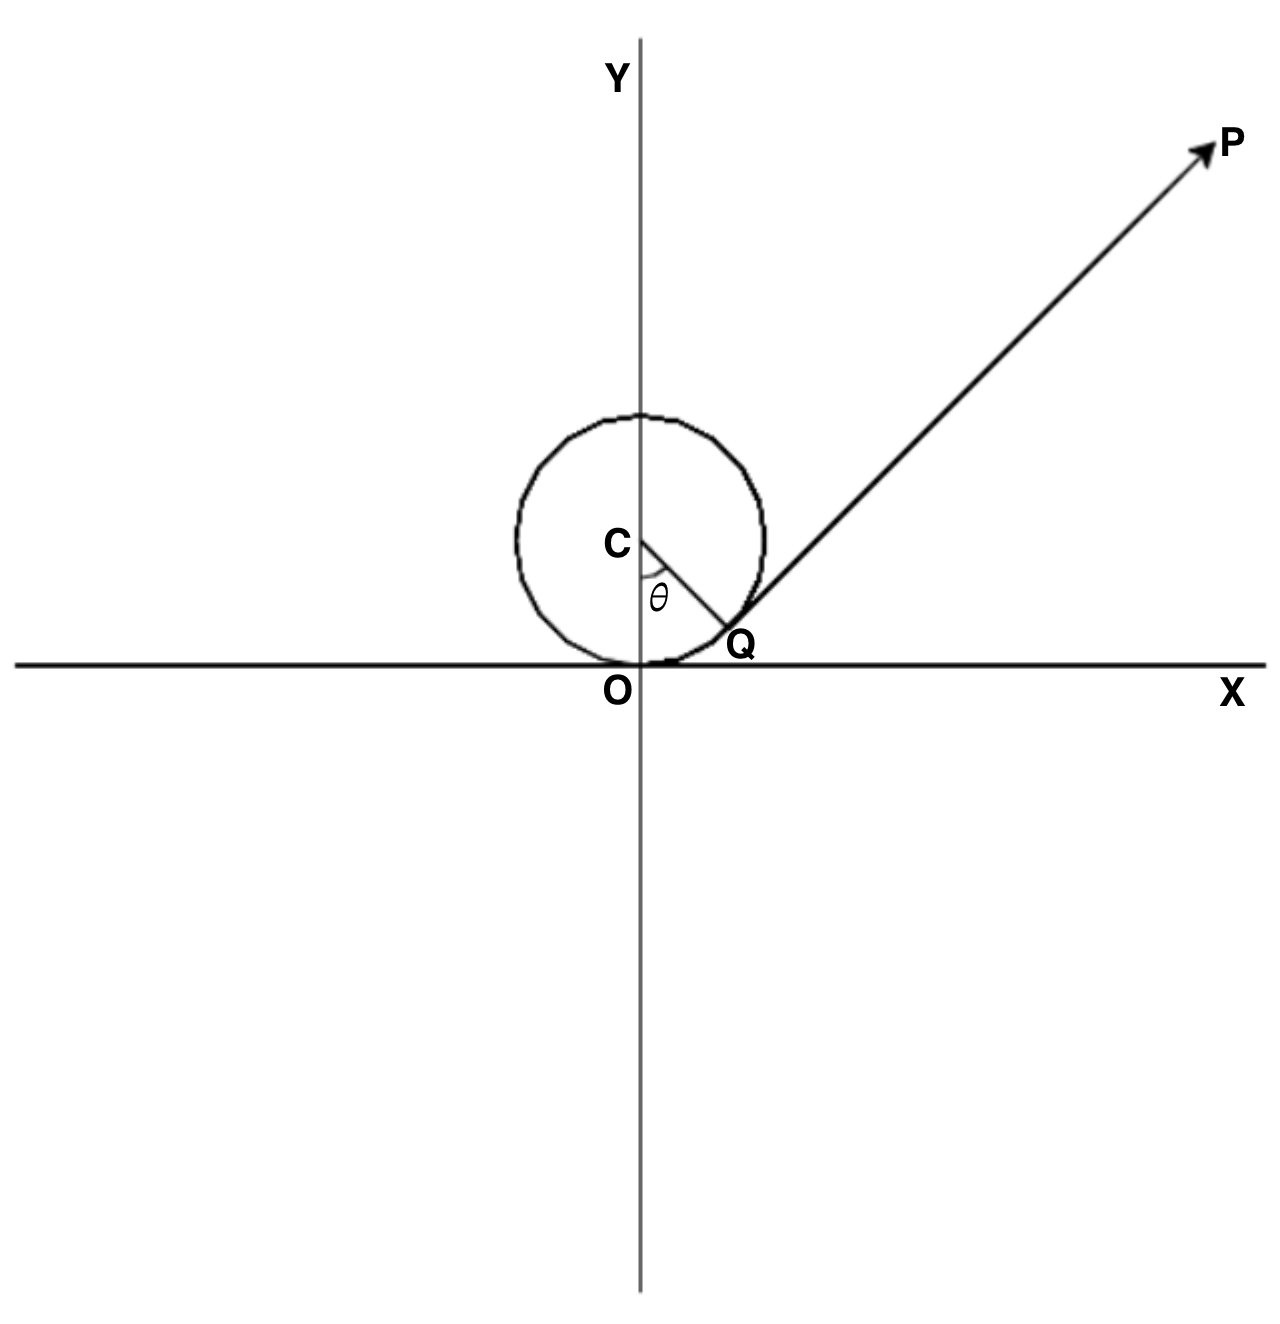
\includegraphics[scale=0.5]{equation-setup}
\centering
\end{figure}

I created the above diagram using a Python program. The program is saved at \texttttilde\texttt{/projects/miscellaneous-stuff/goat-grazing-problem/first-known-goat-grazing-problem/equation-setup.py}.

In the diagram, the circle represents the circular fence the horse is tied to. The radius of the circle is $r$. The horse is tied at the origin $O$. To find the equation of the curve traced by the maximum extent of the rope when the horse is going counterclockwise around the fence, we will take a point $Q$ on the circle and consider the tangent $QP$ at that point. $OQP$ represents the rope. So, the length of $QP$ is equal to the difference between the length of the rope (which is $2 \pi r$) and the length of the arc OQ. We'll find a parameterized equation of the traced curve. We'll use $\theta$, the angle of the arc $OQ$, as the parameter. Let the coordinates of $P$ be $(x, y)$. So, we'll find equations for $x$ and $y$ in terms of $\theta$.

The coordinates of the point $Q$ are $(r \sin \theta, r(1 - \cos \theta))$. The length of $QP$ is equal to $2 \pi r - r \theta$.

When $0 \le \theta \le 2 \pi$, the angle made by $QP$ with the positive $X$ direction is $\theta$. So, $x = (2 \pi r - r \theta) \cos \theta + r \sin \theta$ and $y = (2 \pi r - r \theta) \sin \theta + r(1 - \cos \theta)$.

We can similarly find the equation of the curve traced by the maximum extent of the rope when the horse is going clockwise around the fence. Here, we will again parameterize the equation by the angle of the arc whose length is equal to the length of the rope that is in contact with the circle. We will denote this angle by $\varphi$ to avoid confusion with the parameter $\theta$ which we used in the previous case.

When $0 \le \varphi \le \pi$, $x = (2 \pi r - r \varphi)\cos(\pi - \varphi) - r \sin \varphi = -(2 \pi r - r \varphi)\cos \varphi - r \sin \varphi$ and $y = (2 \pi r - r \varphi) \sin(\pi - \varphi) + r(1 - \cos \varphi) = (2 \pi r - r \phi)\sin \varphi + r(1 - \cos \varphi)$. And when $\pi < \varphi \le 2 \pi$, $x = (2 \pi r - r \varphi)\cos(3 \pi - \varphi) + r \sin(2 \pi - \varphi) = -(2 \pi r - r \varphi)\cos \varphi - r \sin \varphi$ and $y = (2 \pi r - r \varphi)\sin(3 \pi - \varphi) + r (1 - \cos(2 \pi - \varphi) = (2 \pi r - r \varphi)\sin \varphi + r(1 - \cos \varphi)$. So, the equation of the curve traced by the maximum extent of the rope is given by $x = -(2 \pi r - r \varphi)\cos \varphi - r \sin \varphi$ and $y = (2 \pi r - r \varphi)\sin \varphi + r(1 - \cos \varphi)$ with $0 \le \varphi \le 2 \pi$.

Now, let's find the points of intersection of the two curves. We need the points of intersection to determine the proper limits for integration so we can ensure that the area overlapped by the two curves is taken into account exactly once. At a point of intersection, we would have two tangents to the circular fence -- one formed by the rope as the horse is going clockwise and the other formed by the rope as the horse is going counterclockwise. This means that $\varphi = \theta$ at a point of intersection. If we equate the $x$-coordinates of the two curves and then substitute $\theta$ for $\varphi$, we get $(2 \pi r - r \theta)\cos \theta + r \sin \theta = -(2 \pi r - r \theta)\cos \theta - r \sin \theta$. This can be simplified to get $(2 \pi - \theta)\cos \theta + \sin \theta = 0$. Herein lies the difficulty in solving this problem exactly. This is a transcendental equation. I'm not sure if it can be solved exactly. In any case, finding an exact solution of that equation seems to be difficult. Without knowing the points of intersection exactly, we cannot compute the area we're interested in exactly. I think this is probably why Mr. Heath resorted to using numerical methods to solve the problem.

In any case, now that we have the equations for the curves traced by the maximum extent of the rope, we can plot them and see what they look like.

\begin{figure}[h]
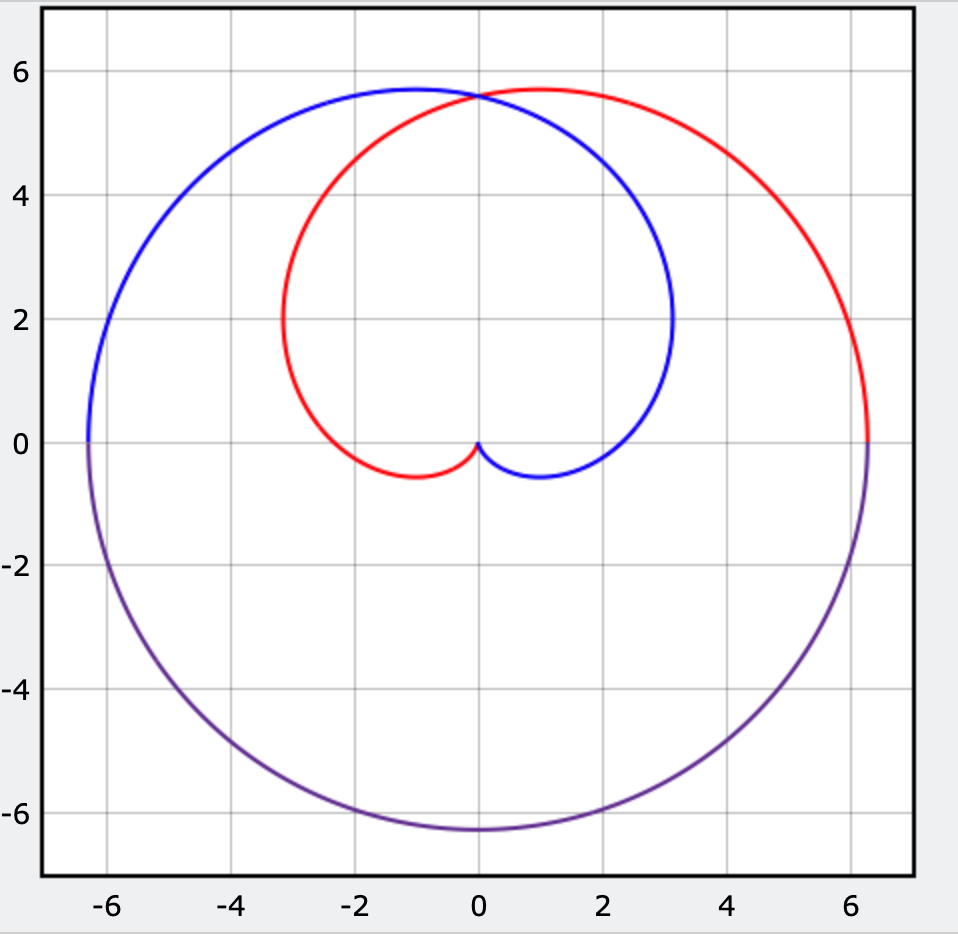
\includegraphics[scale=0.7]{curves-traced-by-rope.png}
\centering
\end{figure}

In the above graph, the red curve is the curve the rope traces when the horse is grazing above the $X$-axis and going around the fence in counterclockwise direction, while the blue curve is the curve traced by the rope when it is going around the fence in clockwise direction while grazing above the $X$-axis. The purple curve is the curve traced by the rope when the horse is grazing below the $X$-axis and it's a semi-circle.

I created this graph using VPython. The code is saved at \texttttilde\texttt{/projects/miscellaneous-stuff/goat-grazing-problem/first-known-goat-grazing-problem/rope-curve.py}. You can run the code online at \url{https://trinket.io/glowscript}.

\end{document}
